\documentclass[10pt]{article}

\usepackage[margin=0.75in]{geometry}
\usepackage{amsmath, amssymb}
\usepackage{graphicx}
\usepackage[T1]{fontenc}
\usepackage{inconsolata}
\usepackage{titlesec}
\usepackage{fancyhdr}
\usepackage{microtype}
\usepackage{tikz}
\usetikzlibrary{arrows.meta,positioning,calc}

\graphicspath{{../}}

\setlength{\parindent}{0pt}
\setlength{\parskip}{4pt}
\setlength{\tabcolsep}{4pt}
\renewcommand{\baselinestretch}{1.05}

\titleformat{\section}{\ttfamily\normalsize\bfseries\MakeUppercase}{\thesection}{0.6em}{}
\titlespacing*{\section}{0pt}{8pt}{2pt}
\titleformat{\subsection}{\ttfamily\small\MakeUppercase}{\thesubsection}{0.6em}{}
\titlespacing*{\subsection}{0pt}{6pt}{2pt}

\pagestyle{fancy}
\fancyhf{}
\renewcommand{\headrulewidth}{0pt}
\renewcommand{\footrulewidth}{0.5pt}
\fancyfoot[L]{\ttfamily\footnotesize WOOD-GABLE-ROOF-SNOW-LOAD}
\fancyfoot[C]{\ttfamily\footnotesize REV \today}
\fancyfoot[R]{\ttfamily\footnotesize \thepage}

\begin{document}

\noindent
\includegraphics[height=0.7cm]{logo}\hfill
{\ttfamily\normalsize\bfseries\MakeUppercase{Wood Gable Roof Snow Load}}\quad
{\ttfamily\footnotesize\today}
\vspace{4pt}\hrule\vspace{6pt}

\section{Code Equations}

{\ttfamily\footnotesize
SCOPE: $W\leq20\text{'-}0\text{"}$; simply supported prismatic wood rafter or joist spans ridge to eave.
}

ASCE 7-16 Eq. 7.3-1:
\begin{equation}
p_f=0.7C_eC_tI_sp_g
\tag{7.3-1}
\end{equation}

{\ttfamily\footnotesize
\begin{tabular}{@{}ll@{}}
$p_f$ & flat roof snow load, psf \\
$C_e$ & exposure factor, Table 7.3-1 \\
$C_t$ & thermal factor, Table 7.3-2 \\
$I_s$ & snow importance factor, Table 1.5-2 \\
$p_g$ & ground snow load, psf \\
\end{tabular}
}

ASCE 7-16 Eq. 7.4-1:
\begin{equation}
p_s=C_sp_f
\tag{7.4-1}
\end{equation}

{\ttfamily\footnotesize
\begin{tabular}{@{}ll@{}}
$p_s$ & balanced sloped roof snow load, psf \\
$C_s$ & roof slope factor, Section 7.4 \\
\end{tabular}
}

ASCE 7-16 Section 7.6.1 and Figure 7.6-1, narrow roof rafter system:
\begin{equation*}
\text{leeward pressure}=I_sp_g,
\qquad
\text{windward pressure}=0
\end{equation*}

{\ttfamily\footnotesize
\begin{tabular}{@{}ll@{}}
$W$ & horizontal eave-to-ridge distance \\
Narrow roof rafter system & $W\leq20\text{'-}0\text{"}$; simply supported prismatic member spans ridge to eave \\
Code location & Section 7.6.1 prose; load pattern shown in Figure 7.6-1; no equation number \\
\end{tabular}
}

Governing uniform roof snow pressure for this note's scope:
\begin{equation*}
q_u=
\begin{cases}
\max\!\left(p_s,\ I_sp_g\right)
& 0.5{:}12\leq\text{roof slope}\leq7{:}12 \\[3pt]
p_s
& \text{roof slope}<0.5{:}12\ \text{or}\ \text{roof slope}>7{:}12
\end{cases}
\end{equation*}

{\ttfamily\footnotesize
\begin{tabular}{@{}ll@{}}
$q_u$ & governing unfactored uniform roof snow pressure, psf \\
Guard & If the scope condition above is not met, use the general pattern in Section 7.6.1 and Figure 7.6-1 \\
\end{tabular}
}

\section{Two-Path Check}

\begin{center}
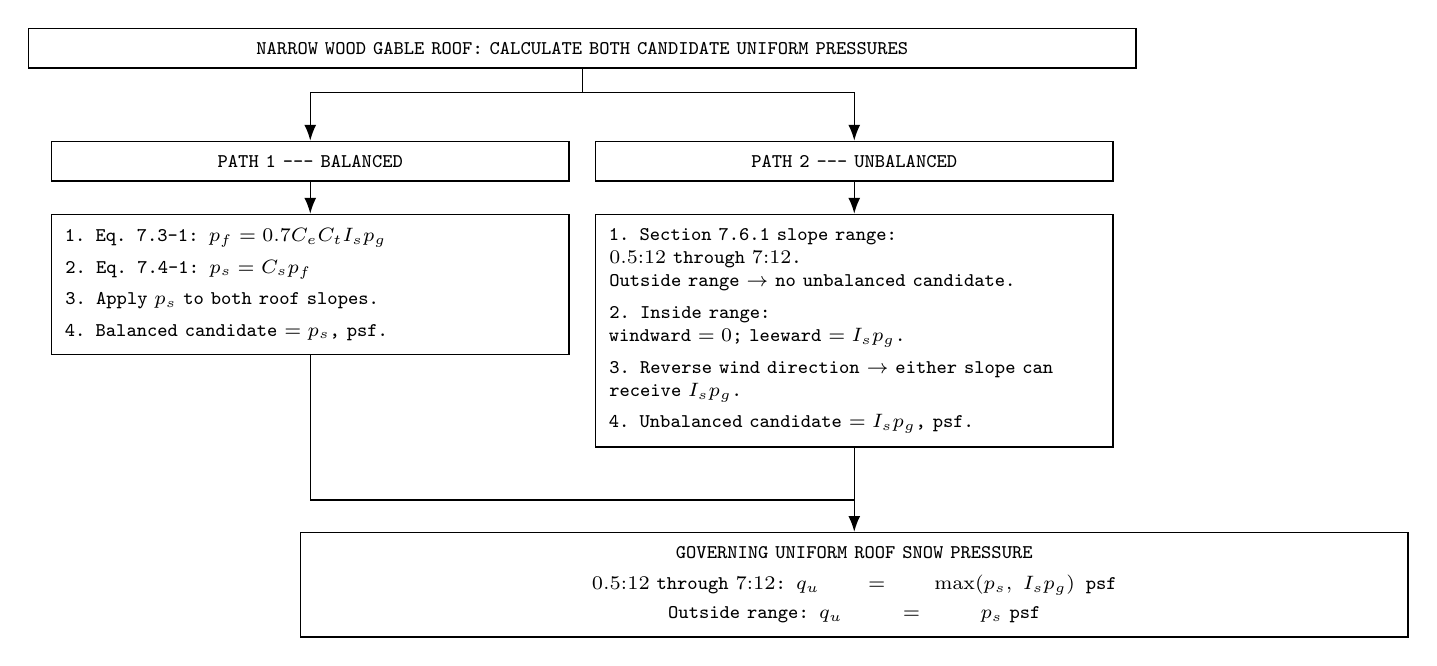
\begin{tikzpicture}[
  font=\ttfamily\scriptsize,
  >=Latex,
  line/.style={draw=black, line width=0.55pt, -{Latex[length=2mm]}},
  branch/.style={draw=black, line width=0.55pt},
  box/.style={draw=black, line width=0.55pt, align=left, inner sep=5pt},
  head/.style={box, font=\ttfamily\scriptsize\bfseries, align=center},
  final/.style={box, font=\ttfamily\scriptsize\bfseries, align=center}
]
\node[head, text width=5.4in] (start) {NARROW WOOD GABLE ROOF: CALCULATE BOTH CANDIDATE UNIFORM PRESSURES};

\node[head, text width=2.45in, below=0.36in of start.south, xshift=-1.36in] (balhead) {PATH 1 --- BALANCED};
\node[head, text width=2.45in, below=0.36in of start.south, xshift=1.36in] (unbalhead) {PATH 2 --- UNBALANCED};

\node[box, text width=2.45in, below=0.16in of balhead] (bal) {
1. Eq. 7.3-1: \(p_f=0.7C_eC_tI_sp_g\)\\[3pt]
2. Eq. 7.4-1: \(p_s=C_sp_f\)\\[3pt]
3. Apply \(p_s\) to both roof slopes.\\[3pt]
4. Balanced candidate \(=p_s\), psf.
};

\node[box, text width=2.45in, below=0.16in of unbalhead] (unbal) {
1. Section 7.6.1 slope range:\\
\(0.5{:}12\) through \(7{:}12\).\\
Outside range \(\rightarrow\) no unbalanced candidate.\\[3pt]
2. Inside range:\\
windward \(=0\); leeward \(=I_sp_g\).\\[3pt]
3. Reverse wind direction \(\rightarrow\) either slope can receive \(I_sp_g\).\\[3pt]
4. Unbalanced candidate \(=I_sp_g\), psf.
};

\node[final, text width=5.4in, below=0.42in of unbal.south] (finish) {
GOVERNING UNIFORM ROOF SNOW PRESSURE\\[3pt]
\(0.5{:}12\) through \(7{:}12\): \(\displaystyle q_u=\max\!\left(p_s,\ I_sp_g\right)\ \text{psf}\)\\[2pt]
Outside range: \(\displaystyle q_u=p_s\ \text{psf}\)
};
\coordinate (join) at ($(finish.north)+(0,0.16in)$);

\draw[line] (start.south) -- ++(0,-0.12in) -| (balhead.north);
\draw[line] (start.south) -- ++(0,-0.12in) -| (unbalhead.north);
\draw[line] (balhead) -- (bal);
\draw[line] (unbalhead) -- (unbal);
\draw[branch] (bal.south) -- (bal.south |- join) -- (join);
\draw[branch] (unbal.south) -- (unbal.south |- join) -- (join);
\draw[line] (join) -- (finish.north);
\end{tikzpicture}
\end{center}

\end{document}
